\documentclass[12pt]{report}
\usepackage[margin=1.0in]{geometry}
\usepackage{graphicx}
\usepackage{caption}
\usepackage{subcaption}

\title{Predicting Sea Levels Using the Actuaries Climate Index}
\date{April 28th, 2017}
\author{Jennifer Mince, Karl Maier, Wesley Merrick,\\ Katie Vervack, Toby Duncan, Katie Kessler}
\begin{document}
	\maketitle
\section*{Abstract} 
\indent	\par The main goal of this project was to use the Actuaries Climate Index data set to answer our central question: how do the seasonal components of high temperature, low temperature, heavy rain, and drought affect the seasonal sea levels in North American regions, and by how much? Rising sea level is a threatening force that greatly impacts local and global environments. Many populations live in an area that would be significantly damaged by impending flooding. Destructive storms, coastal flooding, shoreline erosion, and destroyed ecosystems, industries, and infrastructure are all results of rising sea levels. Roads, bridges, power plants, and other important components of human life are not currently equipped to handle this threat. 
		\par Using this data, our group could help this societal need by introducing a model for the rate at which the sea levels are increasing, and calculating factors that contribute to the increase in levels. The data set has an Actuary Climate Index (ACI) created with the components: frequency of temperatures above the 90th percentile (T90), frequency of temperatures below the 10th percentile (T10), maximum rainfall per month in five consecutive days (Rx5), annual maximum consecutive dry days (CDD), frequency of wind speed above the 90th percentile (WP), and sea level changes (SL). The index is an educational tool designed to help inform actuaries, public policymakers, and the public on changes in these measures over recent decades.  It is an objective measure of changes in extreme weather and changes in sea level relative to the base period of 1961 through 1990. Using the Anaconda interpreter and Python 3, we created code in linear regression and random forest regression models of each component vs. sea level for each region per season. We found some trends for certain seasons or regions, but no trends over components or regions as a whole. Hopefully, our data analysis can be used to further predict sea-level rise if the Actuary Climate Index is updated with more years and features to create larger data sets to make it easier to make predictive conclusions. 

\newpage
 \section* {Introduction} 
		
\indent	\par Our group would like to use the Actuaries Climate Index data set to answer the central question: how do the seasonal components of high temperatures, low temperatures, heavy rain, and drought affect the seasonal sea levels in North American regions and by how much?
		\par The research we want to conduct is both important and relevant to the societal need of knowing what causes sea levels to rise and predicting future measurements to be better prepared for future problems. Higher sea levels have a significant impact on both local and global environments. Rising levels can cause destructive storms to move closer inland and as a result, there is more coastal flooding. \textquotedblleft€œIn the United States, almost 40 percent of the population lives in relatively high-population-density coastal areas, where sea level plays a role in flooding, shoreline erosion, and hazards from storms" (NOAA). Rising seas threaten the infrastructure used by industries and businesses, such as roads, bridges, power plants, and oil wells. The coastline of the United States is heavily populated and the risk of rising sea levels causes many problems. \textquotedblleft Approximately 25 million people live in an area vulnerable to coastal flooding"€ (EPA). The U.S. economy, transportation, and many ecosystems are threatened by the impending flooding that comes with the rising levels. Integral coastal activities including marine transportation of goods, resource extraction, and tourism help to generate \textquotedblleft€œ58\% of the national gross domestic product" (EPA). Transportation in the United States is substantially affected by coastal flooding, especially roads. In low-lying communities, the streets are first to be flooded because they are lower than the surrounding land (Titus). The current drainage systems for these roads are not efficient enough to handle increased frequency of flooding due to rising sea levels. 
		\par Using this data, our group could help this societal need by introducing a model for the rate at which the sea levels are increasing, and calculating factors that contribute to the increase in levels. The data set has an Actuary Climate Index (ACI) created with the components: frequency of temperatures above the 90th percentile (T90), frequency of temperatures below the 10th percentile (T10), maximum rainfall per month in five consecutive days (Rx5), annual maximum consecutive dry days (CDD), frequency of wind speed above the 90th percentile (W), and sea level changes (SL). It is an objective measure of changes in extreme weather and changes in sea level relative to the base period of 1961 through 1990. This index is an educational tool designed to help inform actuaries, public policymakers, and the general public on changes in these measures over recent decades (Actuary Climate Index). Our group will create our own ACI using the seasonal values for T90, T10, Rx5, and CDD to see how they affect the sea level changes. 
	
\section* {Existing Conclusions} 
		
\indent	\par After researching the various data science studies that were conducted using the ACI data set, only two other studies were found. One focused on using the data set to build a risk index for areas where economic losses from disasters (i.e.. floods, droughts, etc)  would be higher than other areas. This index was then going to be used by insurance companies to help set rates for the regions. The other was focused on expanding the data set to account for the UK and Europe. Besides these two studies, however, there wasn't any other relevant research that used the ACI data set. Because of this, the search was expanded to research that used just some of the individual data sets that together composed the ACI. Even in these further searches, there were not really any relevant data science studies, but rather lots of papers that simply analyzed the data instead. Overall, after all this research into other data science using the ACI data set, it is safe to conclude that our particular data science study will be answering a question that has not been answered before in another study.
		
\section* {Cleaning the Data} 

\indent	\par The Actuaries Climate Index data set needed to be cleaned up for our team to effectively and efficiently utilize it for our model. In order to clean up the data, we first needed to understand which variables we wanted to keep as well as determine what each of the variables meant. We decided to keep  the temperature above the 90th percentile, below the 10th percentile, consecutive dry days, rainfall maximum for 5 days, and sea level. Our group thought that these variables were crucial to change in sea level. Since the Central Arctic (CAR) and Midwest (MID) regions had no sea level data so we excluded it from the final clean data set. The CAR region consisted of the Northern Territories and Nunavut. The MID territory consisted of Iowa, Illinois, Indiana, Minnesota, Michigan, Missouri, Ohio, Wisconsin. We are trying to predict how sea level is affected and it would be impossible to predict with out the data for sea level. 
		\par The group excluded the monthly variable sheets in addition to those two regions because  we wanted to focus on the seasonal components. The seasonal components are divided into 4 seasons: Winter (December, January, February), Spring (March, April, May), Summer (June, July, August), and Fall (September, October, November). Our group decided to use the seasonal data rather than the monthly data because of how much data there was to process. The data will show a bigger change when split into 4 seasons rather than smaller changes throughout 12 month periods. Now that we had all our data we wanted we needed to add it all into one sheet on excel. Having all the data on one sheet in excel would allow the code to easily import one comma-separated file. When the coding actually started, the one file was more difficult. The one comma-separated file was kept as a master list which was then broken into multiple sheets based on each individual variable. To make the data look cleaner, the original variable names were simplified. For example, the initial variable of ACI\_sealevel\_seasonal\_ALA.csv  was then converted to SL ALA. Initially, the datasets columns were the years while the rows were the actual variables. The columns and rows were then altered so that the years were the rows and the variables were on the columns. Excel has a function built in called Transpose, which allowed an easy flip of the rows and columns. The clean data then allowed us to implement each comma-separated value files in our code.
		\par After cleaning up the data, we needed to adjust the ACI average to account for discarding the wind power and sea level data. We left the sea level data out of our ACI average because we want to use this average to help determine sea level. In the data set, each year is broken into 4 seasons. The previous ACI average was computed by taking the average of T90, T10, Rx5, CDD, W, and SL for each of those seasons by region. They did this using standardized anomalies. That is, an anomaly divided by a standard deviation. \textquotedblleft The standardized anomaly corresponds to how unusual that season's value is, compared to the reference period mean and standard deviation for that season" (Actuary Climate Index). They used the mean (T90 - T10 + Rx5 + CDD + W + SL) to calculate the ACI average. The reason for negating the T10 variable is to make the standard deviation 1 for this component, matching all other variables. We used this formula for the ACI average but removed wind power (W) and sea level (SL). This makes our final formula ACI = (T90 - T10 + Rx5 + CDD)/4.
		
\section* {Data Analysis} 
		
\indent	\par We soon found out that choosing a machine learning algorithm was more difficult than we thought because there are may different algorithms that we could use. We determined that the k-nearest neighbors regression algorithm would not not work with our data. \textquotedblleft K-nearest neighbors predicts the class of a data point based on the majority vote k-nearest neighbors" (Ismail). The closer the data points are to each other, the better the prediction value. Since our data are spread out and not close to each other, we would get a bad prediction value if we used k-nearest neighbors as our predictive model. We then used linear regression and random forest regression on our data to see if there were any positive r-squared, or r$^2$ values. Linear regression lets us analyze relationships between two quantitate variables. This involves finding the best-fitting straight line through the data points. This line is called a regression line (Lane). From this, we can determine the r$^2$ value. R$^2$ determines how close the data are to the regression line. It is always between 0 and 100\%.  Generally, the larger the r$^2$ value the better the model fits the data (Frost). Random forest regression also uses r$^2$. Random forests are a  \textquotedblleft combination of tree predictors where each tree depends on the values of a random vector..." (Walker). This random vector is obtained separately with the same dispersal for all trees in the forest. Basically, a group of ``weak learners" will move together to create a ``strong learner".
	\par We found slight success when using the method of linear regression. We graphed first each of the following variables (cdd, rx5, t10, t90, and average) versus sea level for each region and season and then ran a linear regression method on each of these graphs. Positive $r^2$ values were found for some of these graphs but not all of them. We will discuss the largest $r^2$ values for \textquoteleft CDD vs SL', \textquoteleft Rx5 vs SL', \textquoteleft T10 vs SL', \textquoteleft T90 vs SL' and \textquoteleft AVG vs SL'. The largest $r^2$ value for \textquoteleft CDD vs SL' was found in summer of region CWP with an $r^2$ value of $0.48$ (Figure: \ref{fig:LinearMaxCDD}). The largest $r^2$ value for \textquoteleft RX5 vs SL' was found in winter of region CWP with an $r^2$ value of $0.41$ (Figure: \ref{fig:LinearMaxRX5}). The largest $r^2$ value for \textquoteleft T10 vs SL' was found in winter of region USA with an $r^2$ value of $0.72$ (Figure: \ref{fig:LinearMaxT10}). The largest $r^2$ value for \textquoteleft T90 vs SL' was found in summer of region SPL with an $r^2$ value of $0.35$ (Figure: \ref{fig:LinearMaxT90}). Lastly, the largest $r^2$ value for \textquoteleft AVG vs SL' was found in winter of region USA an $r^2$ value of $0.59$ (Figure: \ref{fig:LinearMaxAVG}).
	
	\begin{figure}[ht]
\centering 
\begin{subfigure}{.5\textwidth}
\centering
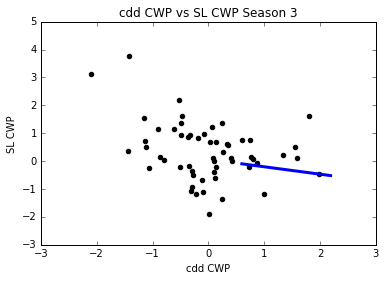
\includegraphics[scale = .5]{CDDLinearMaxS3CWP048.png}
\caption{$r^2 = 0.48$}
\label{fig:LinearMaxCDD}
\end{subfigure}%
\begin{subfigure}{.5\textwidth}
\centering
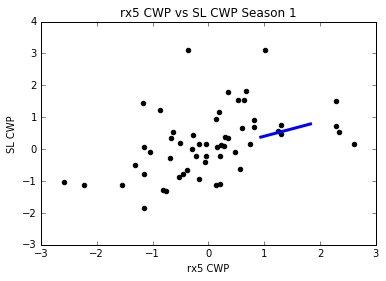
\includegraphics[scale = .5]{RX5LinearMaxS1CWP051.png}
\caption{$r^2 = 0.51$}
\label{fig:LinearMaxRX5}
\end{subfigure}
\begin{subfigure}{.5\textwidth}
\centering
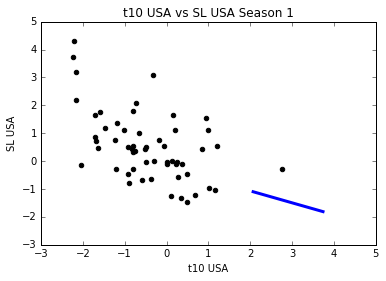
\includegraphics[scale = .5]{T10LinearMaxS1USA072.png}
\caption{$r^2 = 0.72$}
\label{fig:LinearMaxT10}
\end{subfigure}%
\begin{subfigure}{.5\textwidth}
\centering
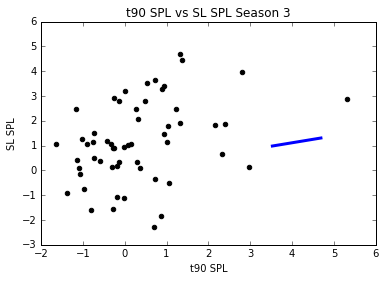
\includegraphics[scale = .5]{T90LinearMaxS3SPL035.png}
\caption{$r^2 = 0.35$}
\label{fig:LinearMaxT90}
\end{subfigure}
\begin{subfigure}{.5\textwidth}
\centering
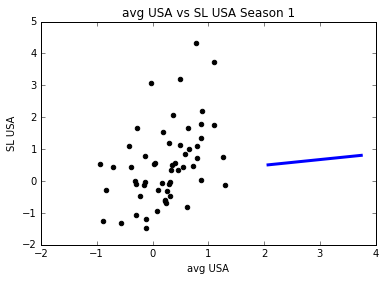
\includegraphics[scale = .5]{AVGLinearMaxS1USA059.png}
\caption{$r^2 = 0.59$}
\label{fig:LinearMaxAVG}
\end{subfigure}
\caption{\label{fig:example}Maximum Linear Regression $r^2$ Values}
\end{figure}

	
	
	
	
	
	






\end{document}
